\documentclass[utf8, russian, aspectratio=1610]{beamer}

\usepackage[utf8]{inputenc}
\usepackage[russian]{babel}
\usepackage{hyperref}
\usepackage{graphicx}
\usepackage{listings}
\usepackage{ucs}
\usepackage{clrscode}
\usepackage{minted}

\makeatletter
\newcommand{\minted@write@detok}[1]{%
  \immediate\write\FV@OutFile{\detokenize{#1}}}%

\newcommand{\minted@FVB@VerbatimOut}[1]{%
  \@bsphack
  \begingroup
    \FV@UseKeyValues
    \FV@DefineWhiteSpace
    \def\FV@Space{\space}%
    \FV@DefineTabOut
    %\def\FV@ProcessLine{\immediate\write\FV@OutFile}% %Old, non-Unicode version
    \let\FV@ProcessLine\minted@write@detok %Patch for Unicode
    \immediate\openout\FV@OutFile #1\relax
    \let\FV@FontScanPrep\relax
%% DG/SR modification begin - May. 18, 1998 (to avoid problems with ligatures)
    \let\@noligs\relax
%% DG/SR modification end
    \FV@Scan}
    \let\FVB@VerbatimOut\minted@FVB@VerbatimOut

\renewcommand\minted@savecode[1]{
  \immediate\openout\minted@code\jobname.pyg
  \immediate\write\minted@code{\expandafter\detokenize\expandafter{#1}}%
  \immediate\closeout\minted@code}
\makeatother

\lstset{
    extendedchars=\true,
    inputencoding=utf8x
}

\usetheme{Warsaw}
\usecolortheme{lily}
\useoutertheme[subsection=false]{smoothbars}
\useinnertheme{circles}
\setbeamertemplate{footline}[page number]{}
\setbeamertemplate{navigation symbols}{}

\renewcommand{\figurename}{} 

\title{Архитектура ЭВМ}
\subtitle{Лекция 6. Системные вызовы}
\author{к.ф.-м.н. Филонов Павел Владимирович \newline filonovpv@gmail.com}
\date{}


\institute[МГТУ ГА] 
{
    Московский Государственный Технический Университет \\
    Гражданской Авиации
}
\begin{document}
\begin{frame}[noframenumbering, plain]
    \titlepage
\end{frame}
\begin{frame}{Содержание}
    \begin{itemize}
        \item Взаимодействие с операционной системой (ОС)
        \item Прерывания процессора
        \item Системные вызовы
        \item Соглашения об системных вызовах в разных ОС
    \end{itemize}
\end{frame}
\begin{frame}{Взаимодействие с ОС}

    {\bf Системный вызов} (англ. system call) в программировании и вычислительной технике — обращение прикладной программы к ядру операционной системы для выполнения какой-либо операции.
        \begin{figure}
        \centering
        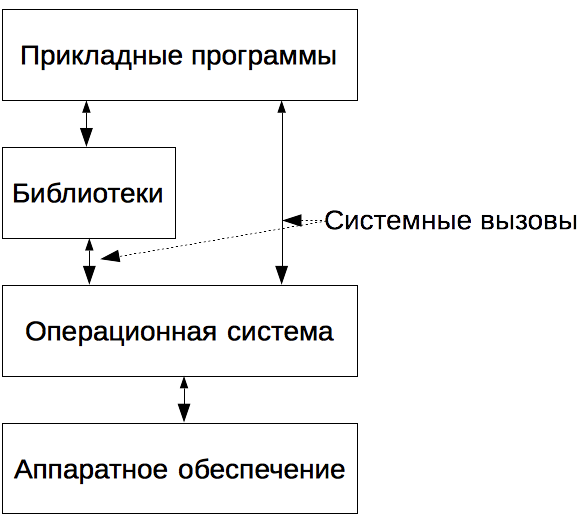
\includegraphics[width=0.5\linewidth]{fig/layers.png}
    \end{figure}
\end{frame}

\begin{frame}{Прерывания процессора}
    \begin{itemize}
        \item внешние (аппаратные)
        \item внутренние (ловушки)
        \item программные (системные вызовы)
    \end{itemize}
\end{frame}

\begin{frame}{Внешние прерывания}

    Данный тип прерывания используется аппаратным обеспечением
    (таймер, контроллер внешнего носителя, сетевая карты и т.д.)
    для сигнализации ЦП об наступлении какого-либо события (срабатывание таймера,
    завершение операции записи, приход сетевого пакета и т.д.)
    \begin{figure}
        \centering
        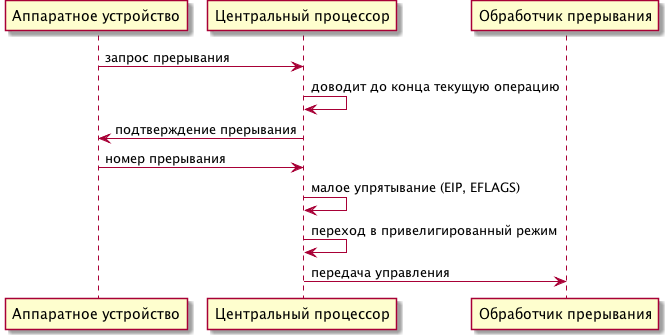
\includegraphics[width=0.8\linewidth]{fig/hardware-interrupt.png}
    \end{figure}
\end{frame}

\begin{frame}{Внутренние прерывания}

    Данный тип прерываний используется ЦП для передачи управления обработчикам его
    собственных внутренних событий (деление на ноль, ошибка сегментации и т.д.).
    \begin{figure}
        \centering
        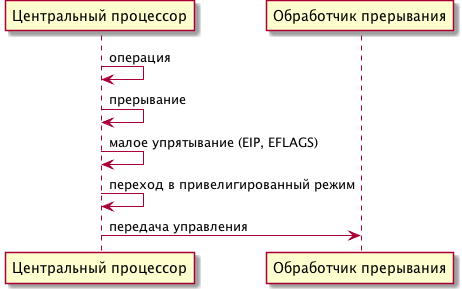
\includegraphics[width=0.6\linewidth]{fig/traps.png}
    \end{figure}
\end{frame}

\begin{frame}{Программные прерывания}

    Используются для передачи управления из прикладной программы в ОС (системные вызовы)
    \begin{figure}
        \centering
        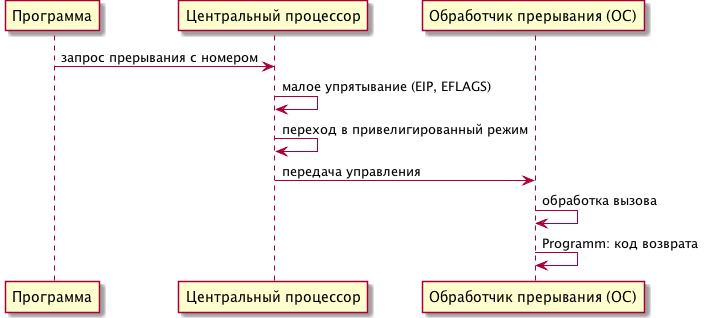
\includegraphics[width=0.8\linewidth]{fig/syscalls.png}
    \end{figure}
\end{frame}

\begin{frame}{Соглашение об системных вызовах в ОС Linux}

    \begin{itemize}
        \item номер системного вызова передается через {\tt eax}
        \item параметры передаются через следующие регистры:
        \begin{itemize}
            \item {\tt ebx, ecx, edx, esi, edi}
        \end{itemize}
        \item системный вызов осуществляется через прерывание по номеру 0x80
        \begin{itemize}
            \item {\tt int 0x80}
        \end{itemize}
        \item результат выполнения возвращается через  {\tt eax}
        \begin{itemize}
            \item результат в диапазоне от {\tt 0xfffff000} до {\tt  0xffffffff} сигнализирует об ошибке
        \end{itemize}
    \end{itemize}
\end{frame}

\begin{frame}[fragile]{Пример: системный вызов {\tt exit}}

Используется для завершения работы программы. В качестве параметра принимает целое число --- код завершения. Любое число отличное от нуля означает неудачное завершение программы.

\begin{minted}[linenos]{nasm}
; exit(0) 
mov eax, 1 ; 1 - номер системного вызова exit
mov ebx, 0 ; 0 - значение параметра (нормальное завершение программы)
int 0x80   ; обращение к прерыванию номер 0x80 
\end{minted}
\end{frame}

    \begin{frame}[fragile]{Пример: системный вызов {\tt write}}
    Используется для записи данных. В качестве параметров принимает:
    \begin{enumerate}
        \item номер файлового дескриптора для вывода;
        \item адрес участки памяти, который необходимо записать;
        \item число байт, которое необходимо записать.
    \end{enumerate}

\begin{minted}[linenos]{nasm}
section .data
    msg db "Hello, world!", 10
    len equ $ - msg
section .text
_start:
    ; write(1, msg, len);
    mov eax, 4   ; 4 - номер системного вызова write
    mov ebx, 1   ; 1 - номер файлового дескриптора,
                 ; который связан со стандартным потоком вывода
    mov ecx, msg ; адрес первого байта строки
    mov edx, len ; длина строки
    int 0x80     ; обращение к прерыванию номер 0x80 
\end{minted}
\end{frame}
\begin{frame}[fragile]{Пример: системный вызов {\tt read}}

    Используется для чтения данных. В качестве параметров принимает:
    \begin{enumerate}
        \item номер файлового дескриптора для записи
        \item адрес участка памяти, куда необходимо записать данные;
        \item максимальное число байт, которое можно прочитать.
    \end{enumerate}
    Возвращает код ошибки или число успешно прочитанных байт. Если возвращается $0$, 
    то это означает, что достигнут <<конце файла>>.

\begin{minted}[linenos]{nasm}
section .bss
    buf resb 128
section .text
_start:
    ; read(0, buffer, 128)
    mov eax, 3   ; 3 - номер СВ read
    mov ebx, 0   ; 0 - номер файлового дескриптора,
                 ; который связан со стандартным потоком ввода
    mov ecx, buf ; в какой участок памяти записать данные
    mov edx, 128 ; максимальное число байт, которое можно прочитать
    int 0x80
\end{minted}
\end{frame}

\begin{frame}[fragile]{Соглашение об системных вызовах в ОС FreeBSD}
    \begin{itemize}
        \item номер системного вызова записывается в регистре {\tt eax};
        \item параметры передаются через стек;
        \item вызов осуществляется в специальной функции {\tt kernel}.
    \end{itemize}
\begin{minted}[linenos]{nasm}
kernel:
    int 0x80
    ret

write:
    push dword len
    push dword msg
    push dword 1
    mov eax, 5
    call kernel
    add esp, 12
\end{minted}
\end{frame}

\begin{frame}[fragile]{Использование команды {\tt sysenter}}

    Является более быстрой версией {\tt int 0x80}
    \begin{itemize}
         \item номер системного вызова сохраняется в {\tt eax};
         \item параметры сохраняются в регистрах {\tt ebx, ecx, edx, esi, edi}
         \item на стеке сохраняется адрес возврата;
         \item на стеке сохраняются регистры {\tt ecx, edx, ebp};
         \item адрес верхушки стека сохраняется в {\tt ebp};
         \item выполняется машинная команда {\tt sysenter};
         \item возвращаемое значение сохраняется в {\tt eax}.
    \end{itemize}
\end{frame}

\begin{frame}[fragile]{Пример использования {\tt sysenter}}
\begin{minted}[linenos]{nasm}
_start:
    ; write(1, msg, len)
    mov eax, 4
    mov ebx, 1
    mov ecx, msg
    mov edx, len
    push dword write_ret
    push ecx
    push edx
    push ebp
    mov ebp, esp
    sysenter

write_ret:
    ; ...
\end{minted}
\end{frame}

\begin{frame}[fragile]{Использование команды {\tt syscall}}

    Используется в наборе машинных команд x86\_64
    \begin{itemize}
         \item номер системного вызова сохраняется в {\tt rax};
         \item номера системных вызовов отличаются от x86;
         \item параметры сохраняются в регистрах {\tt rdi, rsi, rdx, r10, r8, r9};
         \item выполняется машинная команда {\tt syscall};
         \item возвращаемое значение сохраняется в {\tt rax}.
    \end{itemize}
\begin{minted}[linenos]{nasm}
_start:
    ; write(1, msg, len)
    mov rax, 1 ; 1 - номер СВ write для системы команд x86_64
    mov rdi, 1
    mov rsi, msg
    mov rdx, len
    syscall
\end{minted}
\end{frame}

\begin{frame}{Резюме}
    \begin{itemize}
        \item Определение и типы прерываний:
        \begin{itemize}
            \item внешние;
            \item внутренние;
            \item программные.
        \end{itemize}
        \item Программы взаимодействуют с ОС посредством программных прерываний (системных вызовов)
        \item Примеры системных вызовов:
        \begin{itemize}
            \item {\tt exit};
            \item {\tt write};
            \item {\tt read}.
        \end{itemize}
        \item Соглашения об системных вызовах:
        \begin{itemize}
            \item {\tt int 0x80} для Linux;
            \item {\tt int 0x80} для FreeBSD;
            \item {\tt sysenter} для Linux;
            \item {\tt syscall} для Linux x86\_64.
        \end{itemize}
    \end{itemize}
\end{frame}
\end{document}